\subsection{Sujet}

Il va s'agir dans ce projet STL d'étudier la programmation sur les drones dans le cadre des activités robotiques du M2 STL dont les réalisations reposent sur des robots terrestres. Ce projet est donc un moyen d'investigation sur les possibilités offertes par un robot aérien pour un éventuel changement de support robotique.

\paragraph{}
Pour cela, le problème a été posé d'une manière ludique en demandant la réalisation d'un jeu mobile multi-joueur. Selon les données envoyées par les différents joueurs, qui seront centralisées, le drone se mettra en mouvement vers une certaine direction. L'idée de départ est la conception d'un jeu de rythme de type \textit{Guitar Hero}\footnote{Série de jeux vidéo de rythme éditée par \textit{Activision}}.

\begin{figure}[h]
\begin{center}
\fbox{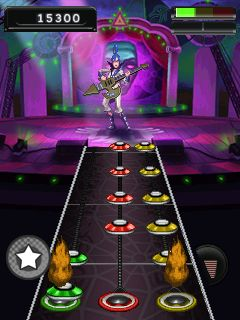
\includegraphics[scale=0.4]{images/guitar_hero.jpg}}
\end{center}
\end{figure}

\paragraph{}
Un environnement client-serveur va être mis en place : les joueurs, à partir de leur application mobile, représentent les clients et se connecteront à un serveur hébergé sur un ordinateur dont le rôle sera de rassembler et traiter les scores des joueurs. A partir de ces données, le serveur communiquera avec le drone pour le piloter vers l'un des joueurs. 

\paragraph{}
Plusieurs objectifs clés ont ainsi été définis durant le projet :
\begin{itemize}
\item Mettre en place un client/serveur
\item Concevoir un jeu mobile
\item Communiquer avec le drone
\item Commander le drone
\end{itemize}